\chapter{$5e^{x+y}$(CDS)}
\label{chapter-cern_math_explorer}
In this chapter we present our solution called $5e^{x+y}$(CDS). We present the key points of our system, and how they are related to previous built systems.

\section{Features Extraction}
Our main goal is to develop a system that compliments the already available search capabilities in Invenio and in particular the CDS instance. Our system was developed on top of the  the Apache Solr/Lucene framework. CDS already uses Solr as a search engine layer, so developing $5e^{x+y}$(CDS) using this technology supposed a reasonable choice. One of the main steps while building an IR tool, is understanding the data and what kind of features can be extracted from it: If the system is based on text, then tasks as stemming, handling of synonyms, misspelling and so on, such be taken into consideration; if the system being developed is based on images, then examples of features can be histograms of colors, geometrical features and so on. During the literature review, we discovered that most of the projects handled the notational aspects of the expressions, that is, the real naming of the terms in a given equation and each project developed its own set of heuristics to handle the structural component. 


\subsection{Notational Features}
Notational features correspond to the elements that relate to the actual naming of the variables, constants and numeric quantities found in an equation. Here we extract tokens that represent single leaf nodes (E.g. <mi>, <mn>, <mo> tags), and simple constructs like subscript and superscript elements, fractions, roots.
We also extract bi-grams and tri-grams as analogue to that is done for text indexing in current systems.

After examining a set of documents from our dataset, we identified some heuristics that could be applied to improve the recall of our system:

\subsubsection{Unicode Normalizing} 
The first issue we discovered is that because of the big wide of different characters to represent the possible mathematical symbols, there is need for an automatic way to match different possible variations of a single character. An example of this situation is specification of an natural number, sometimes denoted by the letter N. In this case, at least three different common representations were identified: $ N = 1 $ (Using character with unicode code point 0x004e), $\mathcal{N} = 1$ (0xd835 0xdc41 or in latex expressed as \lstinline|\mathcal{N}|) and $\mathbb{N} = 1$ (0x2115 or in latex expressed as \lstinline|\mathbb{N}|). \\
  For addressing this situation, we rely on the Unicode equivalence framework. In the unicode specification, sometimes the same character have two or more different code-points because of backwards compatibility with other encoding standards or because the same character has different essential meanings. Another group of equal characters with different code-points are pre-combined characters such as the Latin letter \~{N} which has Unicode point 0x00D1 and also is the sequence of code-points  0x004E (Latin letter N) and 0x0303 (the combining character tilde). Taking this sample into account, Unicode defines the character composition and decomposition operations as replacing the decomposed representation with the pre-composed one and vice-versa. Finally, Unicode defines two types of equivalences between characters: Canonical and compatible. Canonical equivalent characters are assumed to have the same appearance and meaning. Compatible ones are allowed to have slightly different graphical representations but the same meaning in some contexts. One example of compatible equivalent characters is the Roman number 12 {\unicodefontⅫ} with code-point 0x216b and the sequence of characters XII with codepoints 0x0058 0x0049 0x0049. Taking into account the composition or decomposition of characters and the canonical or compatible equivalences, Unicode specifies 4 different forms of a given character:
  \begin{itemize}
  \item NFD: Normalization Form Canonical Decomposition
  \item NFC: Normalization Form Canonical Composition
  \item NFKD: Normalization Form Compatibility Decomposition
  \item NFKC: Normalization Form Compatibility Composition
  \end{itemize}
  
Table \ref{unicode_characters} presents a small list of troubling characters classes that were identified in our datasets.

\begin{longtable}{|m{4cm}|>{\centering\arraybackslash}m{2.15cm}|>{\centering\arraybackslash}m{1.65cm}|>{\centering\arraybackslash}m{1.65cm}|>{\centering\arraybackslash}m{1.65cm}|>{\centering\arraybackslash}m{1.65cm}|}
\hline 
\textbf{Character Name} & \textbf{Visual Rendering} & \textbf{NFC} & \textbf{NFD} & \textbf{NFKC} & \textbf{NFKD} \\ 
\hline 
LATIN CAPITAL LETTER A & A & 0x41 & 0x41 & 0x41 & 0x41 \\ 
\hline 
LATIN CAPITAL LETTER A WITH MACRON & \={A} & 0x100 & 0x41 0x304 & 0x100 & 0x41 0x304 \\
\hline 
LATIN CAPITAL LETTER A WITH RING ABOVE & \r{A} & 0xc5 & 0x41 0x30a & 0xc5 & 0x41 0x30a \\
\hline 
ANGSTROM SIGN (0x212b) &	\r{A} &	0xc5 &	0x41 0x30a &	0xc5 &	0x41 0x30a \\
\hline
LATIN CAPITAL LIGATURE IJ &	IJ &	0x132 &	0x132 &	0x49(I) 0x4a(J) &	0x49 0x4a \\
\hline
CYRILLIC CAPITAL LIGATURE A IE & {\unicodefont Ӕ} &	0x4d4 &	0x4d4 &	0x4d4 &	0x4d4 \\
\hline
LATIN CAPITAL LETTER AE	& {\unicodefont Ӕ}	& 0xc6	& 0xc6	& 0xc6	& 0xc6 \\
\hline
DOUBLE-STRUCK CAPITAL N	& {\unicodefont ℕ}	& 0x2115 & 0x2115 & 0x2115 & 0x4e \\
\hline
LATIN CAPITAL LETTER N	& N & 0x4e	& 0x4e & 	0x4e	& 0x4e \\
\hline 
MATHEMATICAL ITALIC CAPITAL N & $\mathcal{N}$	& 0xd835  0xdc41 &	0xd835  0xdc41 &	0x4e	 & 0x4e \\
\hline 
ROMAN NUMERAL TWELVE	& {\unicodefont Ⅻ}	&0x216b &	0x216b	& 0x58 0x49 0x49 &	0x58 0x49 0x49 \\
\hline
LATIN CAPITAL LETTER X - LATIN CAPITAL LETTER I - LATIN CAPITAL LETTER I &	XII &	0x58 0x49 0x49 &	0x58 0x49 0x49&	0x58(X) 0x49(I) 0x49(I) &	0x58 0x49 0x49 \\
\hline
VULGAR FRACTION ONE QUARTER	& \char"00BC &	0xbc &	0xbc &	0x31(1) 0x2044(/) 0x34(4) &	0x31 0x2044 0x34 \\
\hline
DIGIT ONE - SOLIDUS - DIGIT 4 &	1⁄4 &	0x31  0x2f 0x34 &	0x31 0x2f 0x34	& 0x31 0x2f 0x34 &	0x31 0x2f 0x34\\
\hline
DIGIT ONE - SOLIDUS - DIGIT 4 &	1⁄4 &	0x31  0x2f 0x34 &	0x31 0x2f 0x34	& 0x31 0x2f 0x34 &	0x31 0x2f 0x34\\
\hline
DIGIT ONE - FRACTION SLASH - DIGIT 4 & 1⁄4 &	0x31 0x2044 0x34 &	0x31 0x2044 0x34 &	0x31 0x2044 0x34 &	0x31 0x2044 0x34 \\
\hline
THERE EXISTS	& {\unicodefont ∃}&	0x2203 &	0x2203 &	0x2203 &	0x2203 \\
\hline
THERE DOES NOT EXIST	& {\unicodefont ∄} & 	0x2204	& 0x2203 0x338& 	0x2204 &	0x2203 0x338\\
\hline
LATIN CAPITAL LETTER OPEN E	& {\unicodefont Ɛ} &	0x190 &	0x190 &	0x190 &	0x190 \\
\hline
EULER CONSTANT	& {\unicodefont ℇ} & 0x2107 & 0x2107 & 0x190 & 0x190 \\
\hline
PLANCK CONSTANT	& {\unicodefont ℎ} &	0x210e &	0x210e &	0x68 &	0x68 \\
\hline
LATIN SMALL LETTER H &	h &	0x68 &	0x68 &	0x68 &	0x68 \\
\hline
PLANCK CONSTANT OVER TWO PI	& {\unicodefont ℏ} &	0x210f &	0x210f	& 0x127 &	0x127 \\
\hline
LATIN SMALL LETTER H WITH STROKE & ħ &	0x127	& 0x127	& 0x127	& 0x127 \\
\hline
GREEK CAPITAL LETTER OMEGA	& Ω &	0x3a9 &	0x3a9 &	0x3a9 &	0x3a9 \\
\hline
OHM SIGN & Ω &	0x2126 &	0x2126 &	0x3a9 &	0x3a9 \\
\hline
INTEGRAL & {\unicodefont ∫} &	0x222b &	0x222b &	0x222b &	0x222b \\
\hline
DOUBLE INTEGRAL	& {\unicodefont ∬} & 	0x222c &	0x222c &	0x222b 0x222b &	0x222b 0x222b \\
\hline
CONTOUR INTEGRAL	& {\unicodefont ∮} &	0x222e	 &0x222e &	0x222e &	0x222e \\
\hline
NABLA	& {\unicodefont ∇} &	0x2207	 &0x2207 &	0x2207 &	0x2207 \\
\hline
WHITE DOWN-POINTING TRIANGLE	& {\unicodefont ▽} &	0x25bd	 &0x25bd &	0x25bd &	0x25bd \\
\hline

\caption{Characters with similar glyphs and/or semantics}
\label{unicode_characters}
\end{longtable}


Since our goal is to match as much as possible similar characters, our system employs the NFKD representation of a character. For a given token, we test whether if it is already equal to its NFKD. If not, for all the characters that are not combining nor control characters, we add the token into the same position as the original one.
For example, given the token <mi>\r{A}</mi>, this will lead to the sequence <mi>\r{A}</mi><mi>A</mi> and the token <mi>{\unicodefontⅫ}</mi> will produce <mi>{\unicodefontⅫ}</mi><mi>X</mi><mi>I</mi><mi>I</mi>.

\subsubsection{Operator grouping}
Even though the Unicode normalization step work for a big part of the cases presented in table \ref{unicode_characters}, there are still some groups of characters which would not be matched (Even partially), such as some types of integrals. For addressing these groups, a precomputed table was created for some general groups of operators which have some similar meaning. For each token that belongs to some of this predefined groups, a second token is created identifying the group.
For example the token <mo>{\unicodefont ∮}</mo> is expanded into <mo>{\unicodefont ∮}</mo><mo>INTEGRALS</mo>, similarly the token token <mo>{\unicodefont ∫}</mo> is expanded into <mo>{\unicodefont ∫}</mo><mo>INTEGRALS</mo> and then both will have a partial match in the INTEGRALS token. 
Unicode specification does not define a strict rule to group similar characters based on their semantics. For general operators, we used the grouping provided by Xah Lee in his website\cite{math_groups}.

Figures \ref{integrals} and \ref{less_greater} present lists related of characters for two different categories.

\begin{figure}[h!]
	\centering
	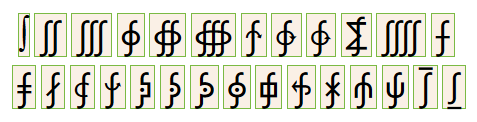
\includegraphics[height=2 cm]{figures/integrals.png}
	\caption{List of different types of integral related characters in Unicode}
	\label{integrals}
\end{figure}

\begin{figure}[h!]
	\centering
	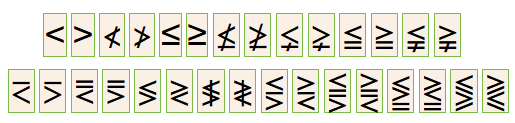
\includegraphics[height=2 cm]{figures/greater_less.png}
	\caption{List of different types of grater/less than related characters in Unicode}
	\label{less_greater}
\end{figure}

\subsubsection{Numeric Approximation} 
Some equations relate specific numeric quantities. While most of the previously explorer systems, handled <mn> tags by only representing them as a constant identifier, this approach is not suitable. A lot of articles in CDS relate to specific experiments under certain conditions, and require a high level of precision in the measurements. However, different experiments of the same phenomenon, can result in different measurements and we wanted to include this variability in our system. To handle this, when a token with a certain numeric quantity is discovered, we apply iterative rounding and index all the different approximations in the same position as the original element. For example the token <mn>2.0135</mn> will produce the following sequence of tokens: <mn>2.0135</mn><mn>2.014</mn><mn>2.01</mn><mn>2.0</mn>. 


\subsection{Structural Features}
The structure of a mathematical expression compliments the information that an be obtained over generic substructures where the naming of the variables is irrelevant.  

\subsubsection{Algebraic structures}
The first set of structures consist on purely algebraic relationships between the expressions.
Inspired by predefined integral tables for different kinds of expressions, we decided to extract from a given equation, whether it has the occurrence of these kind of patterns.
An example of this type of structures would be: $X\textunderscore*(X\textunderscore + A\textunderscore)$ where $X\textunderscore$ and $A\textunderscore$ can be any type of expression. Sample equations matching this pattern can be $C (C+1)$ or $\frac{(\sin{\theta}\cos{\theta})^2}{2a} (\frac{(\sin{\theta}\cos{\theta})^2}{2a} + \tan{\frac{\theta+\phi}{2}})$. This structural analysis of equations is more powerful than the unification of variables and constants proposed in previously discussed projects because these patterns, as shown in the second example, can match an arbitrary complex expression. The drawback of our solution is the need to manually select representative and useful patterns. This selection was done based on standard based tables of integrals similar to the ones that CASs employ to compute them.

\subsubsection{Subscript/Superscript variations}
This set of structures represent common operations that cat appear in a given expression, but its identification is based on notation factors. A simple example of this can be the matrix decomposition $A = VDV^{-1}$ where the actual name of the variables $A$ and $V$ is not meaningful but the real importance is the fact that a given variable appears alongside its inverse in a matrix multiplication form. We would like to assign a partial match to any other kind of this decomposition say $B = MRM^{-1}$. these types of structures live in-between the notational and structural categories but since we identify them using Mathematica, we encompass them as structural features. For this type of structures, we identify simple operations between an element and some possible variations of the same element with some subscript/superscript.

\subsubsection{Specific domain structures}

Additionally, there are common patterns to specific domains which can improve the quality of the retrieved results. Some specific patterns we identified include: $originalParticle \rightarrow subparticle1, subparticle2, subparticle3$ (For representing particle decaying processes) $S = \int^{t2}_{t1} \mathcal{L} dt$ (For an action in terms of its Lagrangian) and $SU(n)$ (For describing special unitary groups). The main drawback of this approach is the need to manually detect, implement and maintain long lists of patterns and for this reason we did not tried to do an exhaustive list of them. 


\section{Development with Lucene/Solr}
This section explains how the described components were implemented in the {\codefont Apache Solr/Lucene} framework.
One focus of our work was to develop a modular system that allowed easily to deploy new heuristics as they were identified. 

Lucene framework defines some key concepts which ultimately are mapped into concrete classes. A {\codefont Document} is the minimum retrieval unit. For $5e^{x+y}$ we could either use a complete article as a document or a single equation. We choose the latter because it makes easier to focus on extracting features from a single equation. A document contains a set of {\codefont fields} which represent different types of information that it can store. Each field has different options such as whether it would be indexed and/or stored. A field can also indicate whether it will be a {\codefont Term Vector}. Our fields are as follow: 
\begin{itemize}
\item math\_notational\_field: This field stores the notational features as a Term Vector. 
\item math\_structural\_field: This field stores the structural features as a Term Vector. 
\item math\_normalized\_notational\_field: This field stores the notational features of the normalized expression as a Term Vector. 
\item filename: This is an auxiliary field which stores the CDS record / article name where the equation was found.
\item number\_occurrences: Another auxiliary field that is used to score final results.
\end{itemize} 

Each field is associated to a particular {\codefont Analyzer}. An analyzer is a specific class that handles an element from a field and groups all the operations that are to be performed. For this purpose we wrote {\codefont SolrNotationalAnalyzer}, {\codefont SolrStructuralAnalyzer} and {\codefont SolrNormalizedNotationalAnalyzer}. 
The Solr prefix is added to make clear the fact that the class extends a {\codefont SolrAnalyzer} which extends a normal lucene {\codefont Analyzer}. 

An analyzer consists of a sequence of {\codefont TokenStrem} elements. Normally an analyzer contains one {\codefont Tokenizer} element (which extends a {\codefont TokenStrem}) that is in charge of creating the Terms that will be stored in the field, and one or more {\codefont TokenFilter} elements which perform operations on the single tokens that were created previously. For the specific cases of SolrNotationalAnalyzer and SolrNormalizedNotationalAnalyzer we created the following classes: 

\begin{itemize}
\item {\codefont MultiplePatternTokenizer}: This class is in charge of applying a set of regular expressions over the given expression in order to extract the single elements that were presented. Lucene incorporates the class {\codefont PatternTokenizer} but it only accepts one regular expression.
\item {\codefont UnicodeNormalizingFilter}: This class receives single tokens and verifies if the token is in Unicode NFKD. In negative case, it emits an additional token in the normalized form.
\item {\codefont SynonymExpandingFilter}: This class verifies if the received token belongs to a predefined category of elements and emits an additional token with it.
\item {\codefont NumericalRoundingFilter}: This class process {\codefont <mn>} tokens. When a number contains a decimal part, it applies the standard rounding mode iteratively and for each one, it emits a token for each step. 
\end{itemize}

{\codefont SolrStructuralAnalyzer } is simpler in its workflow: It consits of a {\codefont StructuralPatternsTokenizer} that tries to find occurrences of the predefined patterns in the expression. For each match, it emits a token with the pattern that was found. 

\section{Integration with Mathematica}
This section describes some aspects that had to be considered while implementing the integration with Mathematica. Our system uses the {\codefont JLink} library to create a connection with the underlying process {\codefont MathKernel}. The main class for communicating java code and {\codefont Mathematica} is {\codefont KernelLink} and the main used method was {\codefont evaluateToOutputForm(String expr, int pageWidth)} where {\codefont expr} is the expression to be evaluated and {\codefont pageWidth} affects the formatting of the result.

\subsubsection{Pattern Extraction}

\subsubsection{Expression simplification}
The second feature that we are interested in is automatic expression simplification.
Mathematica includes different transformations of expressions. These include: {\codefont Simplify} which tries to transform a given equation in an equivalent one but in a reduced form, {\codefont FullSimplify} which is similar to the previous one but tries a higher number of heuristics to apply that can simplify expressions further at the expense of more processing time, {\codefont Factor} to factorize polynomials, {\codefont Refine} which simplifies expressions given certain assumptions about the variables, {\codefont TrigReduce} that tries to apply trigonometric identities to simplify the expression, {\codefont FunctionExpand} that tries to expand special functions in terms of sums and products of other elementary functions. 

The two functions that are more relevant for our work are {\codefont Simplify} and {\codefont FullySimplify} since they apply a combination of the other methods and do not require additional information.

Table \ref{comparison_simplification} presents some sample equations found in some the documents in CDS and the different forms of simplification.

\begin{tabular}{|>{\centering\arraybackslash}m{4.5cm}|>
{\centering\arraybackslash}m{4.5cm}|>
{\centering\arraybackslash}m{4.5cm}|}
\hline
Original Form & {\codefont Simplify} & {\codefont FullSimplify} \\
\hline
\scriptsize{\codefont <math> <mrow> <mrow> <mfrac> <msup> <mi>Φ</mi> <mo>′</mo> </msup> <mrow> <mn>2</mn> <mo>⁢</mo> <mrow> <mo>(</mo> <mrow> <mn>1</mn> <mo>+</mo> <mi>Φ</mi> </mrow> <mo>)</mo> </mrow> </mrow> </mfrac> <mo>+</mo> <mfrac> <mn>1</mn> <mi>r</mi> </mfrac> </mrow> <mo>=</mo> <mn>0</mn> </mrow> </math> }      & \scriptsize{\codefont <math> <mrow> <mrow> <mfrac> <mn>1</mn> <mi>r</mi> </mfrac> <mo>+</mo> <mfrac> <msup> <mi>Φ</mi> <mo>′</mo> </msup> <mrow> <mrow> <mn>2</mn> <mo>⁢</mo> <mi>Φ</mi> </mrow> <mo>+</mo> <mn>2</mn> </mrow> </mfrac> </mrow> <mo></mo> <mn>0</mn> </mrow> </math>}    & \scriptsize{\codefont <math> <mrow> <mrow> <mfrac> <mn>2</mn> <mi>r</mi> </mfrac> <mo>+</mo> <mfrac> <msup> <mi>Φ</mi> <mo>′</mo> </msup> <mrow> <mi>Φ</mi> <mo>+</mo> <mn>1</mn> </mrow> </mfrac> </mrow> <mo></mo> <mn>0</mn> </mrow> </math>}     \\
$\frac{\Phi '}{2 (1+\Phi )}+\frac{1}{r}=0$          & $\frac{1}{r}+\frac{\Phi '}{2 \Phi +2}=0$ & $\frac{2}{r}+\frac{\Phi '}{\Phi +1}=0$       \\

\hline

\scriptsize{\codefont <math> <mrow> <mrow> <mfrac> <mn>1</mn> <mn>2</mn> </mfrac> <mo>⁢</mo> <msup> <mi>x</mi> <mn>2</mn> </msup> <mo>⁢</mo> <mrow> <mi>log</mi> <mo>⁡</mo> <mrow> <mo>(</mo> <mrow> <mn>1</mn> <mo>-</mo> <msup> <mi>e</mi> <mrow> <mo>-</mo> <mrow> <mn>2</mn> <mo>⁢</mo> <mi>x</mi> </mrow> </mrow> </msup> </mrow> <mo>)</mo> </mrow> </mrow> </mrow> <mo>-</mo> <mrow> <mfrac> <mn>1</mn> <mn>2</mn> </mfrac> <mo>⁢</mo> <mi>x</mi> <mo>⁢</mo> <mi>L</mi> <mo>⁢</mo> <msub> <mi>i</mi> <mn>2</mn> </msub> <mo>⁢</mo> <mrow> <mo>(</mo> <msup> <mi>e</mi> <mrow> <mo>-</mo> <mrow> <mn>2</mn> <mo>⁢</mo> <mi>x</mi> </mrow> </mrow> </msup> <mo>)</mo> </mrow> </mrow> <mo>-</mo> <mrow> <mfrac> <mn>1</mn> <mn>4</mn> </mfrac> <mo>⁢</mo> <mi>L</mi> <mo>⁢</mo> <msub> <mi>i</mi> <mn>3</mn> </msub> <mo>⁢</mo> <mrow> <mo>(</mo> <msup> <mi>e</mi> <mrow> <mo>-</mo> <mrow> <mn>2</mn> <mo>⁢</mo> <mi>x</mi> </mrow> </mrow> </msup> <mo>)</mo> </mrow> </mrow> </mrow> </math> }      & \scriptsize{\codefont <math> <mrow> <mfrac> <mn>1</mn> <mn>4</mn> </mfrac> <mo>⁢</mo> <msup> <mi>e</mi> <mrow> <mrow> <mo>-</mo> <mn>2</mn> </mrow> <mo>⁢</mo> <mi>x</mi> </mrow> </msup> <mo>⁢</mo> <mrow> <mo>(</mo> <mrow> <mrow> <mn>2</mn> <mo>⁢</mo> <msup> <mi>x</mi> <mn>2</mn> </msup> <mo>⁢</mo> <msup> <mi>e</mi> <mrow> <mn>2</mn> <mo>⁢</mo> <mi>x</mi> </mrow> </msup> <mo>⁢</mo> <mrow> <mi>log</mi> <mo>⁡</mo> <mo>(</mo> <mrow> <mn>1</mn> <mo>-</mo> <msup> <mi>e</mi> <mrow> <mrow> <mo>-</mo> <mn>2</mn> </mrow> <mo>⁢</mo> <mi>x</mi> </mrow> </msup> </mrow> <mo>)</mo> </mrow> </mrow> <mo>-</mo> <mrow> <mn>2</mn> <mo>⁢</mo> <msub> <mi>i</mi> <mn>2</mn> </msub> <mo>⁢</mo> <mi>L</mi> <mo>⁢</mo> <mi>x</mi> </mrow> <mo>-</mo> <mrow> <msub> <mi>i</mi> <mn>3</mn> </msub> <mo>⁢</mo> <mi>L</mi> </mrow> </mrow> <mo>)</mo> </mrow> </mrow> </math> }    & \scriptsize{\codefont <math> <mrow> <mrow> <mfrac> <mn>1</mn> <mn>2</mn> </mfrac> <mo>⁢</mo> <msup> <mi>x</mi> <mn>2</mn> </msup> <mo>⁢</mo> <mrow> <mi>log</mi> <mo>⁡</mo> <mo>(</mo> <mrow> <mn>1</mn> <mo>-</mo> <msup> <mi>e</mi> <mrow> <mrow> <mo>-</mo> <mn>2</mn> </mrow> <mo>⁢</mo> <mi>x</mi> </mrow> </msup> </mrow> <mo>)</mo> </mrow> </mrow> <mo>-</mo> <mrow> <mfrac> <mn>1</mn> <mn>4</mn> </mfrac> <mo>⁢</mo> <mi>L</mi> <mo>⁢</mo> <msup> <mi>e</mi> <mrow> <mrow> <mo>-</mo> <mn>2</mn> </mrow> <mo>⁢</mo> <mi>x</mi> </mrow> </msup> <mo>⁢</mo> <mrow> <mo>(</mo> <mrow> <mrow> <mn>2</mn> <mo>⁢</mo> <msub> <mi>i</mi> <mn>2</mn> </msub> <mo>⁢</mo> <mi>x</mi> </mrow> <mo>+</mo> <msub> <mi>i</mi> <mn>3</mn> </msub> </mrow> <mo>)</mo> </mrow> </mrow> </mrow> </math>}     \\ 
\scriptsize{ $\frac{1}{2} x^2 \log \left(1-e^{-2 x}\right) - \frac{1}{2} x L i_ 2 \left(e^{-2 x}\right)-\frac{1}{4} L i_ 3 \left(e^{-2 x}\right)$ }          & \scriptsize { \begin{multline}  \frac{1}{4} e^{-2 x} (2 x^2 e^{2 x} \log (1-e^{-2 x})- \notag\\ 2 i_ 2 L x-i_ 3 L)  \end{multline} } & \scriptsize{ $\frac{1}{2} x^2 \log \left(1-e^{-2 x}\right)-\frac{1}{4} L e^{-2 x} \left(2 i_ 2 x+i_ 3\right)$ }      \\

\label{comparison_simplification}
\end{tabular}

\subsubsection{Recursive interpretation}

\subsubsection{Error handling}
Sometimes, after certain time, the connection between {\codefont KernelLink} and {\codefont Mathematica} will be lost launch an exception and following invocations would fails as well.
Also, re-instantiating a KernelLink will yield an Exception. For this scenario, killing the associated processes to Mathematica was necessary with {\codefont killall -s 9 Mathematica; killall -s 9 MathKernel
} or {\codefont taskkill /im Mathematica.exe; taskkill /im MathKernel.exe} depending on the OS the system is running on.

With this, the next creation of a new KernelLink works properly and the subsequent invocations work as expected.

\subsubsection{Timeout Handling}
Unfortunately, checking the quality of a LaTeX document is a difficult job and users have a lot of freedom in the way they write their document since the only visible result is the rendered version. 
One example we found during our work is the following TeX snippet:
\begin{verbatim}
	"\ \varphi\ are\ shown,\ as\ well\ as\ the\ weight\ and\ tension"
\end{verbatim}
A human can easily identify that this corresponds to text and that should be inserted into a proper "mbox" or "text" tag. In this case, the snippet produced the following MathML code:
\small{\codefont <math><mrow><mi>φ</mi><mo></mo><mrow><mi>a</mi><mo></mo>
<mi>r</mi><mo></mo><mi>e</mi></mrow><mo></mo><mrow><mi>s
</mi><mo></mo><mi>h</mi><mo></mo><mi>o</mi><mo></mo><mi>
w</mi><mo></mo><mi>n</mi></mrow><mo>,</mo><mrow><mi>a</m
i><mo></mo><mi>s</mi></mrow><mo></mo><mrow><mi>w</mi><mo
></mo><mi>e</mi><mo></mo><mi>l</mi><mo></mo><mi>l</mi></
mrow><mo></mo><mrow><mi>a</mi><mo></mo><mi>s</mi></mrow>
<mo></mo><mrow><mi>t</mi><mo></mo><mi>h</mi><mo></mo><mi
>e</mi></mrow><mo></mo><mrow><mi>w</mi><mo></mo><mi>e</m
i><mo></mo><mi>i</mi><mo></mo><mi>g</mi><mo></mo><mi>h</
mi><mo></mo><mi>t</mi></mrow><mo></mo><mrow><mi>a</mi><m
o></mo><mi>n</mi><mo></mo><mi>d</mi></mrow><mo></mo><mro
w><mi>t</mi><mo></mo><mi>e</mi><mo></mo><mi>n</mi><mo></
mo><mi>s</mi><mo></mo><mi>i</mi><mo></mo><mi>o</mi><mo><
/mo><mi>n</mi></mrow></mrow></math>
}

Mathematica took around 10 minutes to interpret it.
In the ideal case we would be able to identify the malformed expressions and pass to Mathematica only well-formed equations to be processed but as this simple example shows, that is a very challenging task and may require more work.
As a remedial situation, we used a fixed timeout to stop the processing of a given expression.

\section{Integration with CDS}
Currently the Invenio code-base is being under a deep refactoring and rewriting. CDS currently runs in the stable branch {\codefont master} while the new developments are preferred to be implemented in the new branch {\codefont pu}. 
Our system is deployed as a standalone {\codefont jar} which is added to a Solr instance. Also, some extra configurations should be added. Details on this can be found in appendix \ref{appendix-conf_files}
The communication between Solr and Invenio was through the library {\codefont solrpy}. 
Figure \ref{system_arch} presents the main components of our deployment.

\begin{figure}
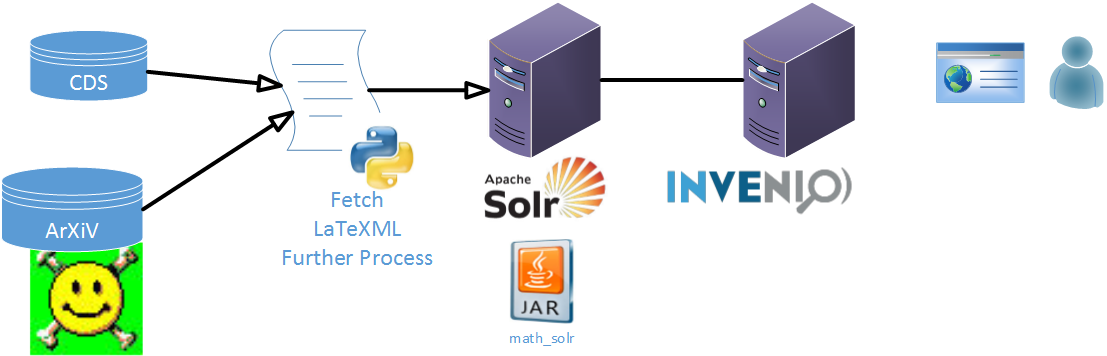
\includegraphics[height=4.2 cm]{visio_drawings/architecture.png}
\label{system_arch}
\caption{High level deployment architecture}
\end{figure}


A demo interface over the {\codefont pu} branch was developed to showcase the system, however to have a complete integration with CDS, a more deep work is required. The demo setup employs the same dataset as used for experimentation. 

\begin{figure}
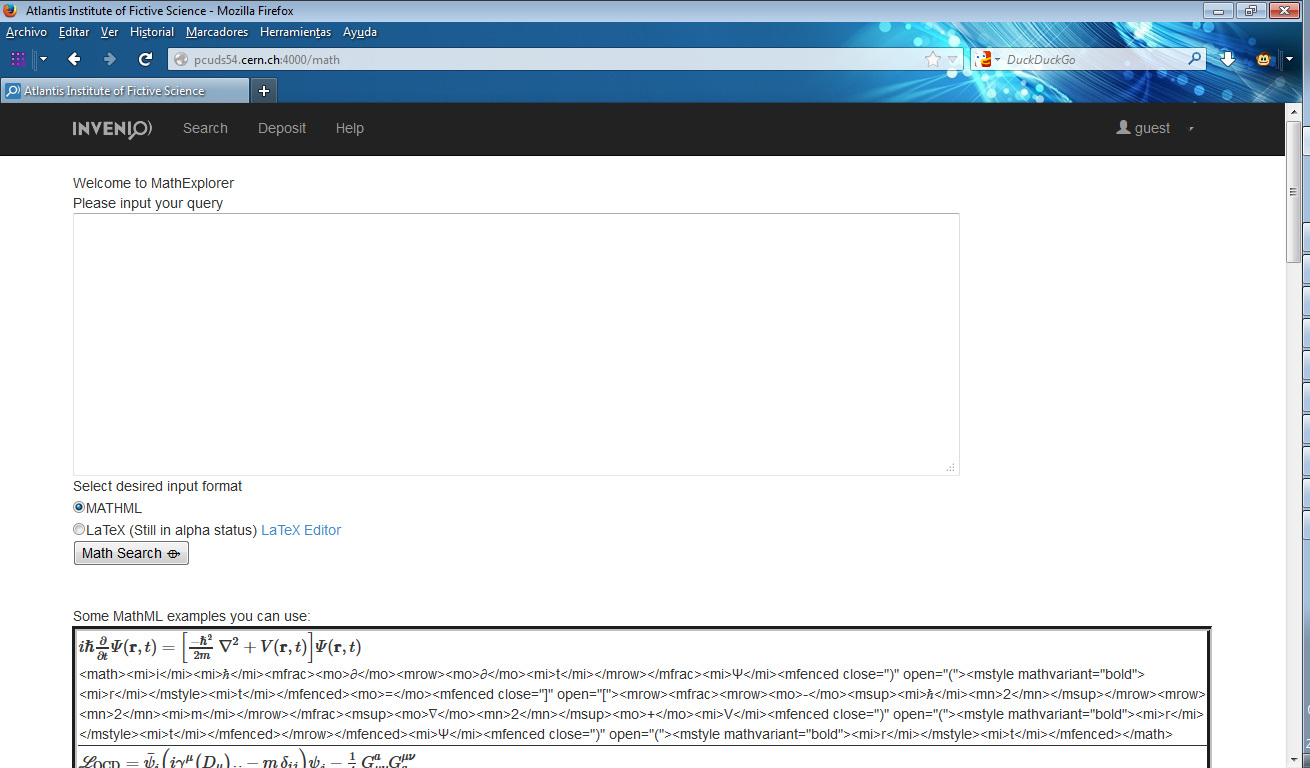
\includegraphics[height=8 cm]{figures/input_interface.png}
\label{input_int}
\caption{Web interface of $5e^{x+y}$: Query input screen}
\end{figure}

\begin{figure}
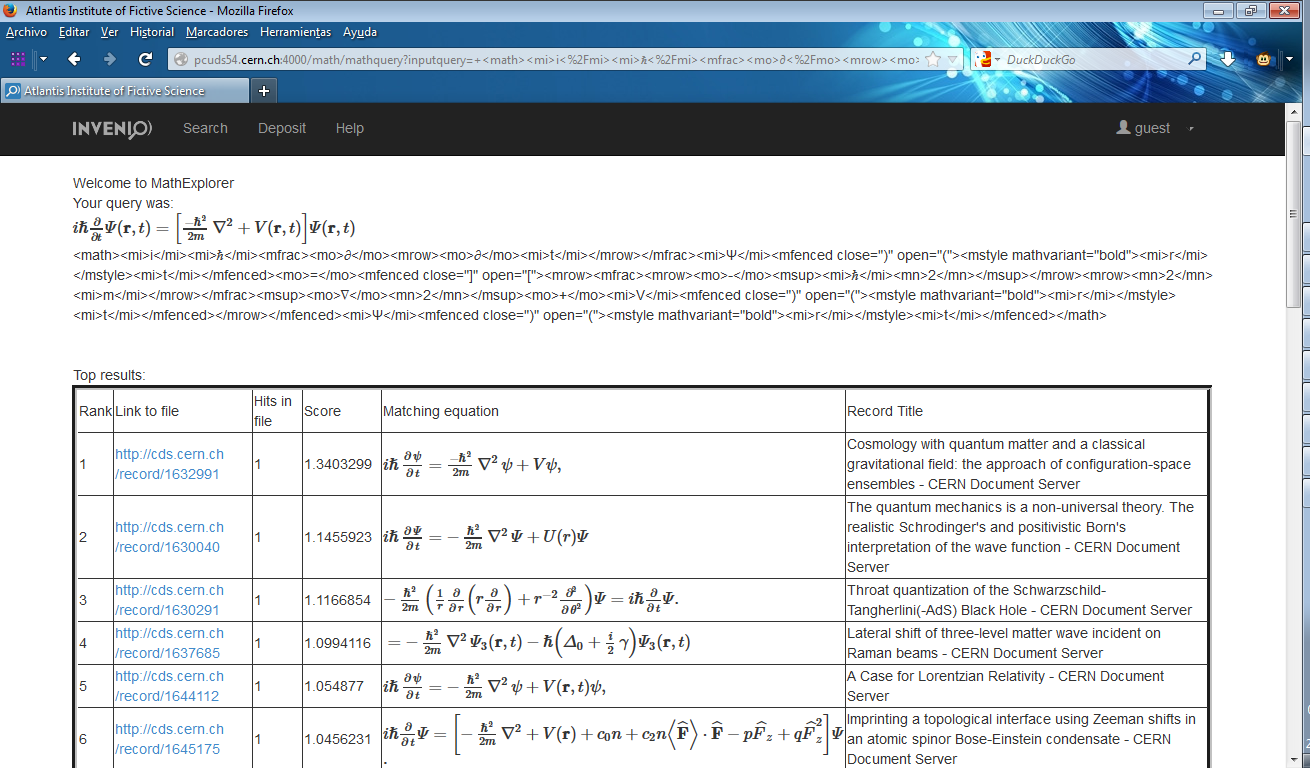
\includegraphics[height=8 cm]{figures/results_interface.png}
\label{results_int}
\caption{Web interface of $5e^{x+y}$: Results screen}
\end{figure}
	
 